% GNUPLOT: LaTeX picture with Postscript
\begingroup
  % Encoding inside the plot.  In the header of your document, this encoding
  % should to defined, e.g., by using
  % \usepackage[cp1252,<other encodings>]{inputenc}
  \inputencoding{cp1252}%
  \makeatletter
  \providecommand\color[2][]{%
    \GenericError{(gnuplot) \space\space\space\@spaces}{%
      Package color not loaded in conjunction with
      terminal option `colourtext'%
    }{See the gnuplot documentation for explanation.%
    }{Either use 'blacktext' in gnuplot or load the package
      color.sty in LaTeX.}%
    \renewcommand\color[2][]{}%
  }%
  \providecommand\includegraphics[2][]{%
    \GenericError{(gnuplot) \space\space\space\@spaces}{%
      Package graphicx or graphics not loaded%
    }{See the gnuplot documentation for explanation.%
    }{The gnuplot epslatex terminal needs graphicx.sty or graphics.sty.}%
    \renewcommand\includegraphics[2][]{}%
  }%
  \providecommand\rotatebox[2]{#2}%
  \@ifundefined{ifGPcolor}{%
    \newif\ifGPcolor
    \GPcolorfalse
  }{}%
  \@ifundefined{ifGPblacktext}{%
    \newif\ifGPblacktext
    \GPblacktexttrue
  }{}%
  % define a \g@addto@macro without @ in the name:
  \let\gplgaddtomacro\g@addto@macro
  % define empty templates for all commands taking text:
  \gdef\gplbacktext{}%
  \gdef\gplfronttext{}%
  \makeatother
  \ifGPblacktext
    % no textcolor at all
    \def\colorrgb#1{}%
    \def\colorgray#1{}%
  \else
    % gray or color?
    \ifGPcolor
      \def\colorrgb#1{\color[rgb]{#1}}%
      \def\colorgray#1{\color[gray]{#1}}%
      \expandafter\def\csname LTw\endcsname{\color{white}}%
      \expandafter\def\csname LTb\endcsname{\color{black}}%
      \expandafter\def\csname LTa\endcsname{\color{black}}%
      \expandafter\def\csname LT0\endcsname{\color[rgb]{1,0,0}}%
      \expandafter\def\csname LT1\endcsname{\color[rgb]{0,1,0}}%
      \expandafter\def\csname LT2\endcsname{\color[rgb]{0,0,1}}%
      \expandafter\def\csname LT3\endcsname{\color[rgb]{1,0,1}}%
      \expandafter\def\csname LT4\endcsname{\color[rgb]{0,1,1}}%
      \expandafter\def\csname LT5\endcsname{\color[rgb]{1,1,0}}%
      \expandafter\def\csname LT6\endcsname{\color[rgb]{0,0,0}}%
      \expandafter\def\csname LT7\endcsname{\color[rgb]{1,0.3,0}}%
      \expandafter\def\csname LT8\endcsname{\color[rgb]{0.5,0.5,0.5}}%
    \else
      % gray
      \def\colorrgb#1{\color{black}}%
      \def\colorgray#1{\color[gray]{#1}}%
      \expandafter\def\csname LTw\endcsname{\color{white}}%
      \expandafter\def\csname LTb\endcsname{\color{black}}%
      \expandafter\def\csname LTa\endcsname{\color{black}}%
      \expandafter\def\csname LT0\endcsname{\color{black}}%
      \expandafter\def\csname LT1\endcsname{\color{black}}%
      \expandafter\def\csname LT2\endcsname{\color{black}}%
      \expandafter\def\csname LT3\endcsname{\color{black}}%
      \expandafter\def\csname LT4\endcsname{\color{black}}%
      \expandafter\def\csname LT5\endcsname{\color{black}}%
      \expandafter\def\csname LT6\endcsname{\color{black}}%
      \expandafter\def\csname LT7\endcsname{\color{black}}%
      \expandafter\def\csname LT8\endcsname{\color{black}}%
    \fi
  \fi
    \setlength{\unitlength}{0.0500bp}%
    \ifx\gptboxheight\undefined%
      \newlength{\gptboxheight}%
      \newlength{\gptboxwidth}%
      \newsavebox{\gptboxtext}%
    \fi%
    \setlength{\fboxrule}{0.5pt}%
    \setlength{\fboxsep}{1pt}%
    \definecolor{tbcol}{rgb}{1,1,1}%
\begin{picture}(7200.00,5040.00)%
    \gplgaddtomacro\gplbacktext{%
      \csname LTb\endcsname%%
      \put(1132,704){\makebox(0,0)[r]{\strut{}$0$}}%
      \csname LTb\endcsname%%
      \put(1132,1527){\makebox(0,0)[r]{\strut{}$0.2$}}%
      \csname LTb\endcsname%%
      \put(1132,2350){\makebox(0,0)[r]{\strut{}$0.4$}}%
      \csname LTb\endcsname%%
      \put(1132,3173){\makebox(0,0)[r]{\strut{}$0.6$}}%
      \csname LTb\endcsname%%
      \put(1132,3996){\makebox(0,0)[r]{\strut{}$0.8$}}%
      \csname LTb\endcsname%%
      \put(1132,4819){\makebox(0,0)[r]{\strut{}$1$}}%
      \csname LTb\endcsname%%
      \put(1264,484){\makebox(0,0){\strut{}$0$}}%
      \csname LTb\endcsname%%
      \put(2087,484){\makebox(0,0){\strut{}$0.2$}}%
      \csname LTb\endcsname%%
      \put(2910,484){\makebox(0,0){\strut{}$0.4$}}%
      \csname LTb\endcsname%%
      \put(3734,484){\makebox(0,0){\strut{}$0.6$}}%
      \csname LTb\endcsname%%
      \put(4557,484){\makebox(0,0){\strut{}$0.8$}}%
      \csname LTb\endcsname%%
      \put(5380,484){\makebox(0,0){\strut{}$1$}}%
    }%
    \gplgaddtomacro\gplfronttext{%
      \csname LTb\endcsname%%
      \put(527,2761){\rotatebox{-270}{\makebox(0,0){\strut{}y (m)}}}%
      \csname LTb\endcsname%%
      \put(5435,2761){\rotatebox{-270}{\makebox(0,0){\strut{}}}}%
      \csname LTb\endcsname%%
      \put(3322,154){\makebox(0,0){\strut{}x (m)}}%
      \csname LTb\endcsname%%
      \put(3322,4819){\makebox(0,0){\strut{}}}%
      \csname LTb\endcsname%%
      \put(-2147483648,924){\makebox(0,0){\strut{}}}%
      \csname LTb\endcsname%%
      \put(132,-110){\makebox(0,0)[l]{\strut{}}}%
      \csname LTb\endcsname%%
      \put(4393,4646){\makebox(0,0)[r]{\strut{}"outputDiagonal.dat"}}%
      \csname LTb\endcsname%%
      \put(5930,704){\makebox(0,0)[l]{\strut{}$0$}}%
      \put(5930,1527){\makebox(0,0)[l]{\strut{}$0.2$}}%
      \put(5930,2350){\makebox(0,0)[l]{\strut{}$0.4$}}%
      \put(5930,3173){\makebox(0,0)[l]{\strut{}$0.6$}}%
      \put(5930,3996){\makebox(0,0)[l]{\strut{}$0.8$}}%
      \put(5930,4819){\makebox(0,0)[l]{\strut{}$1$}}%
      \csname LTb\endcsname%%
      \put(6392,2761){\rotatebox{-270}{\makebox(0,0){\strut{}phi}}}%
      \csname LTb\endcsname%%
      \put(3322,89538){\makebox(0,0){\strut{}}}%
    }%
    \gplgaddtomacro\gplbacktext{%
      \csname LTb\endcsname%%
      \put(1132,704){\makebox(0,0)[r]{\strut{}$0$}}%
      \csname LTb\endcsname%%
      \put(1132,1527){\makebox(0,0)[r]{\strut{}$0.2$}}%
      \csname LTb\endcsname%%
      \put(1132,2350){\makebox(0,0)[r]{\strut{}$0.4$}}%
      \csname LTb\endcsname%%
      \put(1132,3173){\makebox(0,0)[r]{\strut{}$0.6$}}%
      \csname LTb\endcsname%%
      \put(1132,3996){\makebox(0,0)[r]{\strut{}$0.8$}}%
      \csname LTb\endcsname%%
      \put(1132,4819){\makebox(0,0)[r]{\strut{}$1$}}%
      \csname LTb\endcsname%%
      \put(1264,484){\makebox(0,0){\strut{}$0$}}%
      \csname LTb\endcsname%%
      \put(2087,484){\makebox(0,0){\strut{}$0.2$}}%
      \csname LTb\endcsname%%
      \put(2910,484){\makebox(0,0){\strut{}$0.4$}}%
      \csname LTb\endcsname%%
      \put(3734,484){\makebox(0,0){\strut{}$0.6$}}%
      \csname LTb\endcsname%%
      \put(4557,484){\makebox(0,0){\strut{}$0.8$}}%
      \csname LTb\endcsname%%
      \put(5380,484){\makebox(0,0){\strut{}$1$}}%
    }%
    \gplgaddtomacro\gplfronttext{%
      \csname LTb\endcsname%%
      \put(527,2761){\rotatebox{-270}{\makebox(0,0){\strut{}y (m)}}}%
      \csname LTb\endcsname%%
      \put(5435,2761){\rotatebox{-270}{\makebox(0,0){\strut{}}}}%
      \csname LTb\endcsname%%
      \put(3322,154){\makebox(0,0){\strut{}x (m)}}%
      \csname LTb\endcsname%%
      \put(3322,4819){\makebox(0,0){\strut{}}}%
      \csname LTb\endcsname%%
      \put(-2147483648,924){\makebox(0,0){\strut{}}}%
      \csname LTb\endcsname%%
      \put(132,-110){\makebox(0,0)[l]{\strut{}}}%
      \csname LTb\endcsname%%
      \put(4393,4646){\makebox(0,0)[r]{\strut{}"outputDiagonal.dat"}}%
      \csname LTb\endcsname%%
      \put(5930,704){\makebox(0,0)[l]{\strut{}$0$}}%
      \put(5930,1527){\makebox(0,0)[l]{\strut{}$0.2$}}%
      \put(5930,2350){\makebox(0,0)[l]{\strut{}$0.4$}}%
      \put(5930,3173){\makebox(0,0)[l]{\strut{}$0.6$}}%
      \put(5930,3996){\makebox(0,0)[l]{\strut{}$0.8$}}%
      \put(5930,4819){\makebox(0,0)[l]{\strut{}$1$}}%
      \csname LTb\endcsname%%
      \put(6392,2761){\rotatebox{-270}{\makebox(0,0){\strut{}phi}}}%
      \csname LTb\endcsname%%
      \put(3322,94357){\makebox(0,0){\strut{}}}%
    }%
    \gplgaddtomacro\gplbacktext{%
      \csname LTb\endcsname%%
      \put(1132,704){\makebox(0,0)[r]{\strut{}$0$}}%
      \csname LTb\endcsname%%
      \put(1132,1527){\makebox(0,0)[r]{\strut{}$0.2$}}%
      \csname LTb\endcsname%%
      \put(1132,2350){\makebox(0,0)[r]{\strut{}$0.4$}}%
      \csname LTb\endcsname%%
      \put(1132,3173){\makebox(0,0)[r]{\strut{}$0.6$}}%
      \csname LTb\endcsname%%
      \put(1132,3996){\makebox(0,0)[r]{\strut{}$0.8$}}%
      \csname LTb\endcsname%%
      \put(1132,4819){\makebox(0,0)[r]{\strut{}$1$}}%
      \csname LTb\endcsname%%
      \put(1264,484){\makebox(0,0){\strut{}$0$}}%
      \csname LTb\endcsname%%
      \put(2087,484){\makebox(0,0){\strut{}$0.2$}}%
      \csname LTb\endcsname%%
      \put(2910,484){\makebox(0,0){\strut{}$0.4$}}%
      \csname LTb\endcsname%%
      \put(3734,484){\makebox(0,0){\strut{}$0.6$}}%
      \csname LTb\endcsname%%
      \put(4557,484){\makebox(0,0){\strut{}$0.8$}}%
      \csname LTb\endcsname%%
      \put(5380,484){\makebox(0,0){\strut{}$1$}}%
    }%
    \gplgaddtomacro\gplfronttext{%
      \csname LTb\endcsname%%
      \put(527,2761){\rotatebox{-270}{\makebox(0,0){\strut{}y (m)}}}%
      \csname LTb\endcsname%%
      \put(5435,2761){\rotatebox{-270}{\makebox(0,0){\strut{}}}}%
      \csname LTb\endcsname%%
      \put(3322,154){\makebox(0,0){\strut{}x (m)}}%
      \csname LTb\endcsname%%
      \put(3322,4819){\makebox(0,0){\strut{}}}%
      \csname LTb\endcsname%%
      \put(-2147483648,924){\makebox(0,0){\strut{}}}%
      \csname LTb\endcsname%%
      \put(132,-110){\makebox(0,0)[l]{\strut{}}}%
      \csname LTb\endcsname%%
      \put(4393,4646){\makebox(0,0)[r]{\strut{}"outputDiagonal.dat"}}%
      \csname LTb\endcsname%%
      \put(5930,704){\makebox(0,0)[l]{\strut{}$0$}}%
      \put(5930,1527){\makebox(0,0)[l]{\strut{}$0.2$}}%
      \put(5930,2350){\makebox(0,0)[l]{\strut{}$0.4$}}%
      \put(5930,3173){\makebox(0,0)[l]{\strut{}$0.6$}}%
      \put(5930,3996){\makebox(0,0)[l]{\strut{}$0.8$}}%
      \put(5930,4819){\makebox(0,0)[l]{\strut{}$1$}}%
      \csname LTb\endcsname%%
      \put(6392,2761){\rotatebox{-270}{\makebox(0,0){\strut{}phi}}}%
      \csname LTb\endcsname%%
      \put(3322,99176){\makebox(0,0){\strut{}}}%
    }%
    \gplbacktext
    \put(0,0){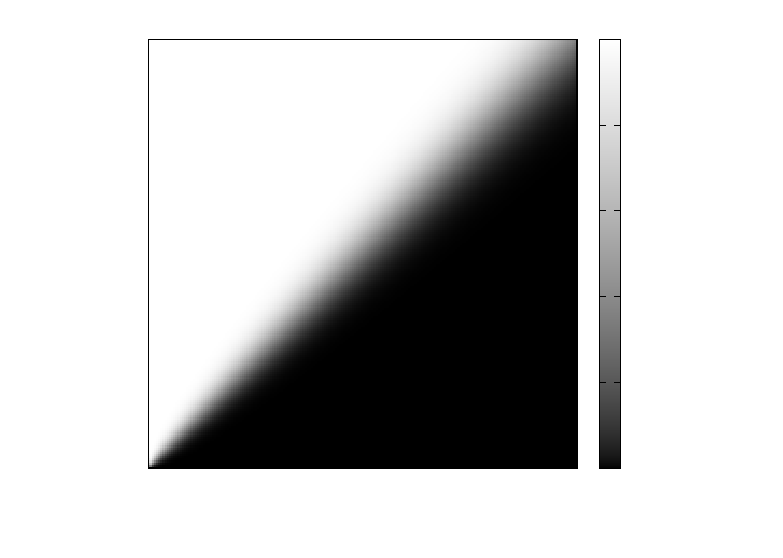
\includegraphics[width={360.00bp},height={252.00bp}]{sections/case_diagonal_flow/test.eps}}%
%    \gplfronttext
  \end{picture}%
\endgroup
